





% Bom dia a todos!

%Bom dia,

% Vamos apresentar o nosso trabalho intitulado ``Classificação Inteligente de Proposições Legislativas'' no qual realizamos uma análise comparativa de modelos de aprendizado de máquina aplicadas à classificação de proposições legislativas".

% Os integrantes deste trabalho somos eu, Ronie Paulucio Porfirio e o Luca Peres Quinta da Guarda.

% Obrigado por estarem aqui e esperamos que aproveitem a apresentação


% Esse é o conteúdo da apresentação. Eu vou iniciar fazendo uma introdução, vou apresentar o problema e os objetivos do trabalho, falar da revisão de literatura e explicar a metodologia.

% Em seguida, o Luca vai apresentar os experimentos conduzidos, os resultados, conclusões e trabalhos futuros


% Vamos apresentar o nosso trabalho intitulado ``Classificação Inteligente de Proposições Legislativas'' no qual realizamos uma análise comparativa de modelos de aprendizado de máquina aplicadas à classificação de proposições legislativas".



% Obrigado por estarem aqui e esperamos que aproveitem a apresentação

% Versao rapida

% Esse é o conteúdo da apresentação. Eu vou apresentar da introdução até a metodologia.

% E o Luca finaliza apresentando resultados, conclusões e trabalhos futuros.


% =========================================================
\section{Introduction}
\begin{frame}
	\frametitle{Introduction}
	\framesubtitle{Business Understanding - Legislative Proposal's Definition and Types}

	\begin{exampleblock}{Legislative Proposal} 
	\begin{itemize}
		\item A \textbf{Legislative Proposal} is any matter subject to deliberation by the Legislative Chamber (CLDF Internal Regulations, art. 129).
	\end{itemize}
	\end{exampleblock}

	% Introdução: Entendendo o Negócio

	% Uma proposição legislativa é toda matéria sujeita à deliberação na Câmara Legislativa.
	% Elas incluem (ler cada uma).


	\begin{exampleblock}{} 
	\textbf{Legislative Proposals can be of the following types:}
	\begin{multicols}{2}
		\begin{itemize}
			\item Proposta de emenda à Lei Orgânica;
			
			\item Projeto de lei complementar;
			
			\item Projeto de lei;
			
			\item Projeto de decreto legislativo;
			
			\item Projeto de resolução;
			
			\item Indicação;
			
			\item Moção;
			
			\item Requerimento;
			
			\item Emenda;
			
			\item Recursos;
		\end{itemize}
	\end{multicols}
	\end{exampleblock}
\end{frame}
% --------------------------------------------------------------------------------------------
\begin{frame}
	\frametitle{Introduction}
	\framesubtitle{Business Understanding - Legislative Proposal's Themes}

	% As proposições são classificadas em um ou mais temas, dentro de um total de 34 temas disponíveis.
	
	% Por exemplo, uma mesma proposição pode ser classificada como: Assunto Social, Saúde e Educação.  
	% Por exemplo, uma mesma proposição pode ser classificada como: Assunto Social, Saúde e Educação.  


	%https://ple.cl.df.gov.br/#/proposicao/buscar	
	\begin{exampleblock}{Legislative Proposals are classified into one or more themes:} 
		\begin{multicols}{3}
			\begin{itemize}
				\scriptsize
				\item Agricultura
				\item Assistência Social
				\item Assunto Fundiário e Ordenamento Territorial
				\item Assunto Social
				\item Cidadania
				\item Ciência e Tecnologia
				\item Combate à Corrupção
				\item Comunicação
				\item Comércio e Serviços
				\item Cultura
				\item Defesa do Consumidor
				\item Desenvolvimento Econômico
				\item Desporto e Lazer
				\item Direitos Humanos
				\item Economia
				\item Educação
				\item Energia
				\item Fiscalização e Governança
				\item Habitação
				\item Incentivos Fiscais e Concessões Públicas
				\item Indústria
				\item Meio Ambiente
				\item Não se aplica
				\item Outro
				\item Previdência Social
				\item Relações Exteriores
				\item Saneamento
				\item Saúde
				\item Segurança
				\item Servidor Público
				\item Trabalho
				\item Transporte e Mobilidade Urbana
				\item Turismo
				\item Urbanismo
				\normalsize
			\end{itemize}
		\end{multicols}
		\textbf{Total:} 34 themes	
	\end{exampleblock}
\end{frame}
% --------------------------------------------------------------------------------------------
\begin{frame}
	\frametitle{Introduction}
	\framesubtitle{Business Understanding - Why Themes?}
	\begin{block}{Thematic Classification Benefits} % Block without title
		\begin{itemize}
			\item Efficient classification of legislative proposals is crucial to \textbf{streamline their analysis} and processing within the legislative process helping to \textbf{determine which committees a proposal should go through}.
					
			% Mas porque realizar essa classificação temática? 
							
			% Uma classificação eficiente ajuda a otimizar o processo legislativo, por exemplo, para determinar em quais comissões uma proposta deve passar.

			\item By categorizing legislative proposals into relevant themes, lawmakers can streamline their analysis, \textbf{allocate resources efficiently}, and \textbf{make informed decisions}. 

			% Ajuda os legisladores a alocar recursos de forma eficiente, melhora a transparência, a manutenção da recuperação precisa de informações, facilita um fluxo legislativo mais organizado e garante uma gestão legislativa eficaz.
			\item This process \textbf{enhances transparency} and facilitates a more \textbf{organized legislative workflow}.	
			% 

					
			\item Thematic classification plays an important role in maintaining \textbf{accurate information retrieval} and \textbf{ensuring effective legislative management}.
			
			% Em resumo, a classificação temática desempenha um papel importante na manutenção da recuperação precisa de informações e na garantia de uma gestão legislativa eficaz.
				
		\end{itemize}
	\end{block}
\end{frame}
% =========================================================
\section{The Problem}
\begin{frame}
	\frametitle{The Problem}
	\framesubtitle{Understanding the problem}
	
	% Qual é o problema?
	
	\begin{alertblock}{Theme ``others'' is growing bigger}
		\begin{itemize}
			\item 	Usually, the author of the proposal is responsible for classifying it into one or more themes.
			
			% A escolha dos temas para classificar uma proposição é geralmente feita pelo autor da proposição.
			
			\item Unfortunately, due to various factors such as ambiguous topics, outdated categories, multidisciplinary nature, \textbf{many propositions end up being classified under the generic theme of ``outro'' (others)}.
			
			% Contudo, infelizmente, devido a diversos fatores, como tópicos ambíguos, categorias desatualizadas e natureza multidisciplinar, muitas proposições acabam sendo classificadas sob o rótulo genérico de “outros”.
			
		\end{itemize}
	\end{alertblock}	
\end{frame}
% --------------------------------------------------------------------------------------------
\begin{frame}
	\frametitle{The Problem}
	\framesubtitle{Understanding the problem}	
	\begin{figure}
		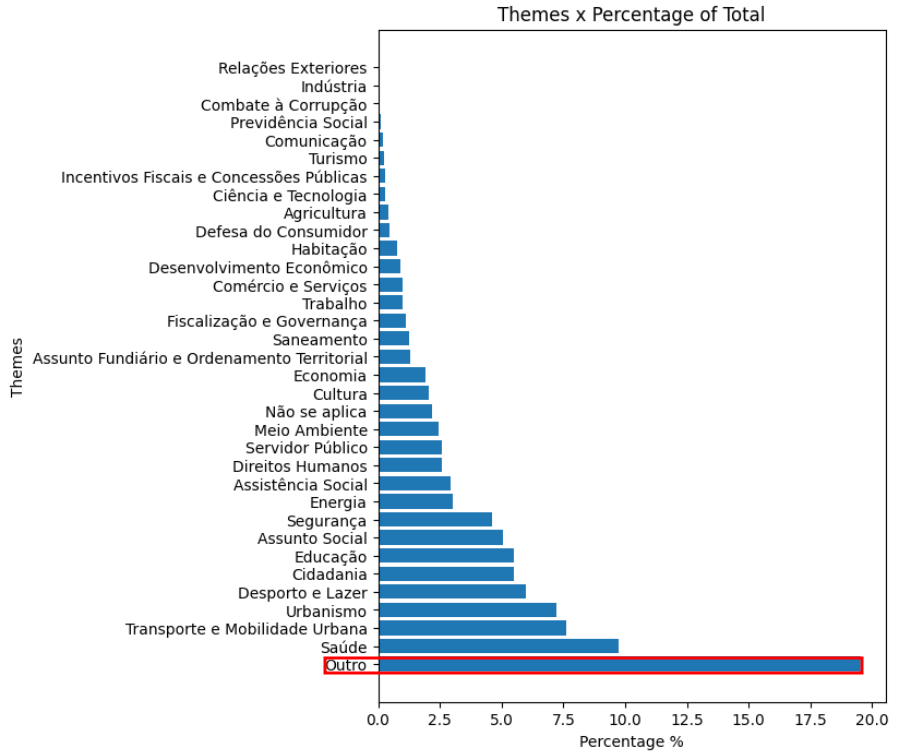
\includegraphics[width=0.6\linewidth]{graphThemes.png}
	\end{figure}

	% Para ilustrar esse problema, nesse gráfico mostramos o percentual do total de proposições classificadas em cada tema até maio de 2024.

	\begin{block}{}
		\scriptsize
		The chart shows that the number of proposals classified under the theme ``outro'' (other) represents almost 20\% of the total. 
	\end{block}	

	% O gráfico mostra que o número de proposições classificadas com o tema "outros" já corresponde a quase 20% do total.

\end{frame}
% --------------------------------------------------------------------------------------------
\begin{frame}
	\frametitle{The Problem}
	\framesubtitle{Problem definition}	

	\begin{alertblock}{The problem is inadequate proposal classification}
		Inadequate classification hinders efficient tracking, analysis, and transparency of legislative activities, making it difficult for both society and lawmakers to understand and oversee the legislative process effectively.
	\end{alertblock}	

	\begin{figure}
		
\includegraphics[width=0.3\linewidth]{problem.jpeg}
	\end{figure}

	% O problema, portanto, é a classificação inadequada de proposições sobre o tema "outros".

	% Essa classificação inadequada dificulta o acompanhamento eficiente, a análise e a transparência das atividades legislativas, tornando desafiador tanto para a sociedade quanto para os legisladores compreender e supervisionar efetivamente o processo legislativo. 
\end{frame}
% =========================================================
\section{Objective}

\begin{frame}
	\frametitle{Objectives}
	\framesubtitle{Primary objective}
	
	\begin{exampleblock}{Primary objective} 
		\begin{itemize}
			\item The primary objective of this study is to \textbf{compare different machine learning models} to determine which model is \textbf{most effective in suggesting more appropriate theme categories for legislative proposals}.
			
			\item The goal is to find \textbf{more suitable themes that better match these proposals}.  
		\end{itemize}
	\end{exampleblock}
	
	\begin{figure}
		
\includegraphics[width=0.3\linewidth]{arrow.jpeg}
	\end{figure}
	
	% Então qual é o objetivo desse trabalho?


		% \item O objetivo principal deste estudo é \textbf{comparar diferentes modelos de aprendizado de máquina} para determinar qual modelo é \textbf{mais eficaz em sugerir categorias de temas mais apropriadas para propostas legislativas.

	
	
	
	
\end{frame}


\begin{frame}
	\frametitle{Objectives}
	\framesubtitle{Disclaimer}
		
	\begin{alertblock}{Attention!} 
		\begin{itemize}
			\item This study \textbf{does not aim to automate the classification process, replace human classification, or compare human classification with machine learning classification}. 
			
			\item Instead, \textbf{the focus is on enhancing the existing categorization process by identifying the best model for suggesting themes for proposals currently classified under the generic label "others."}.
		\end{itemize}
	\end{alertblock}
	
%\item Este estudo não tem como objetivo automatizar o processo de classificação, não tem como objetivo substituir a classificação humana e nem mesmo comparar a classificação humana com a classificação por aprendizado de máquina}.

% \item Em vez disso, \textbf{o foco é melhorar o processo de categorização existente, identificando o melhor modelo para sugerir temas para propostas atualmente classificadas sob o rótulo genérico "outros"}.
	
	
	
\end{frame}

% ----------------------




% =========================================================
\section{Literature review}
\begin{frame}
	\frametitle{Literature review}
	
	\begin{thebibliography}{99} % Beamer does not support BibTeX so references must be inserted manually as below, you may need to use multiple columns and/or reduce the font size further if you have many references
	\footnotesize % Reduce the font size in the bibliography
		\scriptsize
	

		\bibitem[Junior, 2021]{p1}
		J. Andrade Junior, J. Cardoso-Silva, and L. Bezerra (2021)
		\newblock \href{https://core.ac.uk/download/491169432.pdf}{Comparing Contextual Embeddings for	Semantic Textual Similarity in Portuguese}
		\newblock \scriptsize \emph{Anais da X Brazilian Conference on Intelligent Systems} 

		% Na nossa revisão da literatura optamos por evidenciar esses três artigos. 

		% O primeiro nos levou a experimentar a vetorização por embeddings como alternativa ao TF-IDF.
		
		% Os outros dois nos ajudaram na escolher os modelos de classificação de texto experimentados
		
		%\bibitem[Reimers, 2019]{p2}
		%Reimers, Nils and Gurevych, Iryna (2019)
		%\newblock \href{http://arxiv.org/abs/1908.10084}{Sentence-BERT: Sentence %Embeddings using Siamese BERT-Networks}
		%\newblock \emph{Proceedings of the 2019 Conference on Empirical Methods in %Natural Language Processing} 
		%\newblock \emph{Association for Computational Linguistics} 
				

		% https://link.springer.com/article/10.1007/s41133-020-00032-0#citeas
		\bibitem[Huwail, 2022]{p2}
		Alantari, J., Currim, S., Sanghvi, Y. et al. (2022)
		\newblock \href{https://doi.org/10.1016/j.ijresmar.2021.10.011}{An empirical comparison of machine learning methods for text-based sentiment analysis of online consumer reviews}
		\newblock \scriptsize \emph{International Journal of Research in Marketing - Pages 1-19} 

					
		% https://link.springer.com/article/10.1007/s41133-020-00032-0#citeas
		\bibitem[Shah, 2022]{p3}
		Shah, K., Patel, H., Sanghvi, D. et al. (2022)
		\newblock \href{https://doi.org/10.1007/s41133-020-00032-0}{A Comparative Analysis of Logistic Regression, Random Forest and KNN Models for the Text Classification}
		\newblock \scriptsize \emph{Augment Hum Res 5, 12} 


		

		% https://www.sciencedirect.com/science/article/abs/pii/S0022169419310285
		%\bibitem[Yu, 2020]{p4}
		%Yu, Xiang, et al. (2020)
		%\newblock \href{https://doi.org/10.1007/s41133-020-00032-0}{Comparison of support vector regression and extreme gradient boosting for decomposition-based data-driven 10-day streamflow forecasting.}
		%\newblock \scriptsize \emph{Journal of Hydrology 582 (2020): 124293} 
		
		 
		
 
		
		

		
		
		
		
		\normalsize		 

	\end{thebibliography}

	
	
\end{frame}
% =========================================================
\section{Methodology}

\begin{frame}
	\frametitle{Methodology}
	\framesubtitle{CRISP-DM's Methodology}	
	% Utilizamos a metodologia CRISP-DM cujas etapas serão 	apresentadas nos próximos slides.
	\begin{figure}
		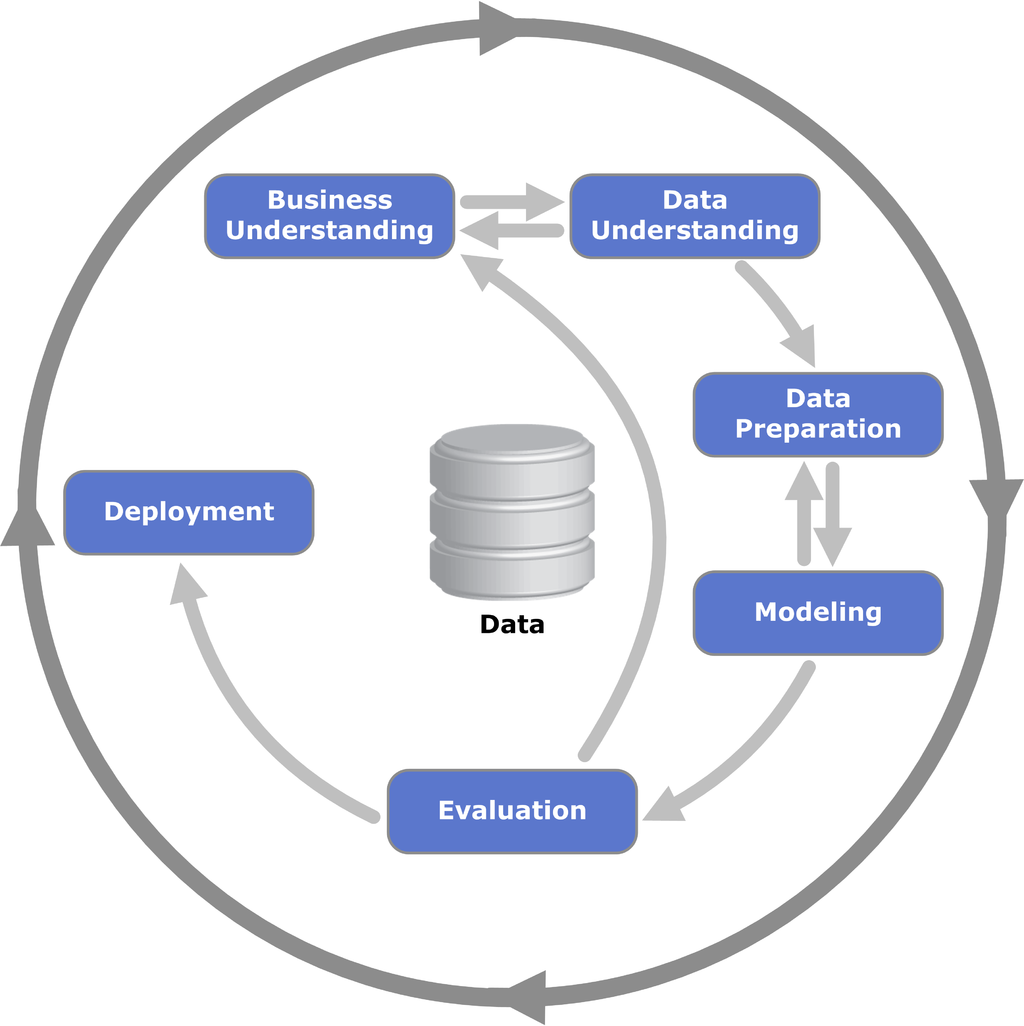
\includegraphics[width=0.5\linewidth]{crispdm.png}
	\end{figure}

	\begin{block}{}
	\scriptsize
		We utilized the CRISP-DM methodology. Its stages will be explained in the following slides.	
	\end{block}	
\end{frame}

% --------------------------------------------------------
\begin{frame}
	\frametitle{Methodology}
	\framesubtitle{1 - Business Understanding}	
	
	\begin{block}{1 - Business Understanding} 
			We have analyzed legislative documents to align our data mining objectives with legislative classification needs.
	\end{block}

	% Na primeira etapa do CRISP-DM "Entendimento do Negócio", nós analisamos diversos documentos para alinhar nossos objetivos de mineração de dados com as necessidades de classificação de preposições legislativas.

	% Por exemplo, a figura (a) mostra um projeto de lei que institui a semana de inteligência artificial a ser realizada anualmente na segunda semana do mês de agosto.
	
	% A figura (b) mostra os principais metadados da proposição: O tipo é Projeto de Lei, o número definitivo é 954/2024 e neste caso ele foi classificado com o tema ``Ciência e Tecnologia''. 

	\begin{figure}
		\centering
		\begin{subfigure}[b]{0.4\textwidth}
			
\includegraphics[width=\textwidth]{plePLExemplo.png}
			\caption{Proposal example}
		\end{subfigure}
		\hspace{0.1\textwidth}
		\begin{subfigure}[b]{0.4\textwidth}
			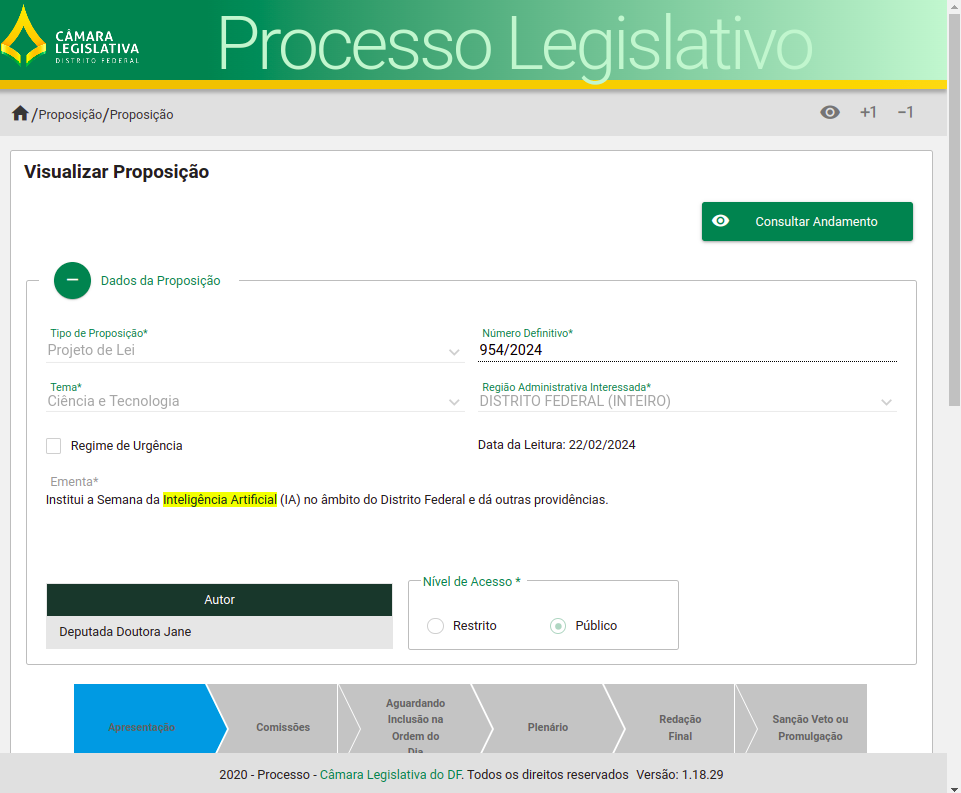
\includegraphics[width=\textwidth]{plePropMetadados.png}
			\caption{Proposal's data}
		\end{subfigure}
	\end{figure}

\end{frame}
%-------------------------------------------------
\begin{frame}
	\frametitle{Methodology}
	\framesubtitle{2 - Data Understanding}	
	\begin{block}{2 - Data Understanding} 
		The dataset contains 22,267 summaries extracted from the ``\textit{Processo Legislativo Eletrônico (PLE)}`` system, covering the period from 2021 to May 2024. Each summary is accompanied by its respective thematic classification.
	\end{block}

	\begin{figure}
		
\includegraphics[width=0.2\linewidth]{lupa.png}
	\end{figure}


	% O conjunto de dados contém 22.267 ementas extraídas do sistema de Processo Legislativo Eletrônico (PLE) abrangendo o período de 2021 a maio de 2024. Cada resumo é acompanhado por sua respectiva classificação temática.

\end{frame}
%-------------------------------------------------
\begin{frame}
	\frametitle{Methodology}
	\framesubtitle{3 - Data Preparation}	

	\begin{block}{3 - Data Preparation} 
		\begin{enumerate}

			\item \textbf{Preprocessing}: We discard data classified under ``outro'' and ``não se aplica'' themes. Then, we perform tokenization, normalization, stopword removal, and lemmatization processes.
			
			\item \textbf{Vectorization}:
			\begin{itemize}
				\item \textbf{Multilingual sentence embedding model} based on the MiniLM architecture, a lightweight and efficient BERT variant with 12 transformer layers, to produce high-quality embeddings that capture the semantic meaning of the text. 
				
				\item \textbf{TF-IDF (Term Frequency-Inverse Document Frequency) model} involves converting text into numerical vectors based on the frequency of terms within a document and across a collection of documents. This approach captures the importance of a term in a document relative to the entire dataset.
			\end{itemize}
		\end{enumerate}
	\end{block}
\end{frame}


% Descartamos dados "outro" e "não se aplica", depois realizamos tokenização, normalização, remoção de stopwords e lematização.

% A Vetorização ocorre usando duas técnicas:
% Embedding baseado na arquiterura MiniLM, para produzir incorporações de alta qualidade.
	
% E o odelo TF-IDF para converter texto em vetores numéricos, capturando a importância dos termos.



%-------------------------------------------------
\begin{frame}
	\frametitle{Methodology}
	\framesubtitle{4 - Modeling: Chosen Models - Part I}	
	
	\begin{block}{4 - Modeling} 
		\begin{enumerate}
			\item \textbf{DummyClassifier}: A \textbf{baseline model} that makes predictions using simple rules and establishes a baseline to \textbf{compare the performance of more complex models}.
			
			\item \textbf{Support Vector Machine (SVM)}: A powerful model that \textbf{finds the hyperplane that best separates the classes in the feature space}. It is  effective for high-dimensional spaces and when the number of dimensions exceeds the number of samples.
			
			\item \textbf{Logistic Regression}: A linear model that \textbf{estimates the probability of a binary outcome based on input features}. It is simple and interpretable, good for linearly separable data and understanding feature importance.
		\end{enumerate}
	\end{block}
\end{frame}

%\item \textbf{DummyClassifier}: Um modelo de base que usa regras simples para comparar o desempenho de modelos mais complexos.

%\item \textbf{Support Vector Machine (SVM)}: Encontra o hiperplano que melhor separa as classes. Eficaz para espaços de alta dimensionalidade.

%\item \textbf{Logistic Regression}: Estima a probabilidade de um resultado binário com base nas características de entrada. 

%\item \textbf{XGBoost (Extreme Gradient Boosting)}: Algoritmo otimizado que constrói um conjunto de árvores de decisão para melhorar o desempenho. Conhecido por alta performance e escalabilidade.

%\item \textbf{Random Forest}: Constrói várias árvores de decisão e agrega suas previsões. Robusto contra overfitting.

%\item \textbf{K-Nearest Neighbors (KNN)}: Classifica pontos de dados com base na classe majoritária de seus k vizinhos mais próximos. Simples e eficaz para conjuntos de dados pequenos.

% ---------------------
\begin{frame}
	\frametitle{Methodology}
	\framesubtitle{4 - Modeling: Chosen Models - Part II}	
	\begin{block}{4 - Modeling (cont...)} 
		\begin{enumerate}
			\setcounter{enumi}{3}
			\item \textbf{XGBoost (Extreme Gradient Boosting)}: An optimized gradient boosting algorithm that \textbf{builds an ensemble of weak learners (typically decision trees) to improve model performance}. Known for high performance, speed, and scalability.
			
			\item \textbf{Random Forest}: An \textbf{ensemble model that constructs multiple decision trees and aggregates their predictions}. Robust against overfitting, good for handling large datasets with higher dimensionality.
			
			\item \textbf{K-Nearest Neighbors (KNN)}: A \textbf{non-parametric model that classifies a data point based on the majority class of its k nearest neighbors}. Simple and intuitive, effective for small datasets with low noise.
		\end{enumerate}
	\end{block}
\end{frame}




%-------------------------------------------------
\begin{frame}
	\frametitle{Methodology}
	\framesubtitle{4 - Modeling: Justification}	
	\begin{alertblock}{Why choose these models?} 
		\begin{enumerate}
			\scriptsize
			\item \textbf{Baseline Comparison}: DummyClassifier provides a benchmark to gauge the performance of more sophisticated models.

			\item \textbf{Linear and Non-Linear Data}: Logistic Regression and SVM cover linear relationships, while Random Forest, XGBoost, and KNN handle non-linear data.

			\item \textbf{Model Performance}: XGBoost and Random Forest are chosen for their strong predictive performance and ability to handle complex datasets.

			\item \textbf{Interpretability}: Logistic Regression is valued for its simplicity and ease of interpretation.

			\item \textbf{Versatility}: SVM, Random Forest, and XGBoost offer versatility across different types of data and problems.

			\item \textbf{Scalability}: XGBoost is particularly chosen for its scalability and efficiency in handling large datasets.
		\end{enumerate}
	\end{alertblock}
\end{frame}



%	DummyClassifier serve como referência para avaliar os modelos mais avançados.
	
% 	Temos modelos para lidar com dados lineares e não lineares.	

%	Alguns vão apresentar alta performance ao lidar com dados complexos.
	
%  E outros facilitam a interpretação, são versáteis e escaláveis quando usados em grandes conjuntos de dados.


% -------------------
	
%	Interpretabilidade com o Logistic Regression sendo valorizado pela sua simplicidade e fácil interpretação.
	
%	\item \textbf{Versatilidade}: SVM, Random Forest e XGBoost são versáteis para diversos tipos de dados e problemas.
	
%	\item \textbf{Escalabilidade}: XGBoost é escolhido pela sua eficiência e escalabilidade em grandes conjuntos de dados.


%-------------------------------------------------
\begin{frame}
	\frametitle{Methodology}
	\framesubtitle{5 - Evaluation}	
	
	\begin{block}{5 - Evaluation} 
			Our evaluation metrics include \textbf{Accuracy}, \textbf{Precision}, \textbf{Recall} and \textbf{F1 score}.
	\end{block}

	\begin{block}{} 
		\begin{itemize}
			\item \textbf{Accuracy} is \textbf{straightforward and easy to understand}.
			\item \textbf{Precision} and \textbf{recall} are more informative when dealing with \textbf{imbalanced classes} because they provide insights into the performance of the minority class, which accuracy might overlook.
			
			\item \textbf{F1 score} gives a \textbf{balance between precision and recall as a single metric} to \textbf{summarize} the model performance.
		\end{itemize}
	\end{block}
\end{frame}

% A quinta etapa da metodologia é a forma de avaliar os resultados

% Nossas métricas de avaliação incluem \textbf{Acurácia}, \textbf{Precisão (Precision)}, \textbf{Revocação (Recall)} e \textbf{F1 Score}.

% A acuracia é a métrica mais elementar, ela é \textbf{direta e fácil de entender}.

%\item \textbf{Precisão} e \textbf{Recall} são mais informativas para \textbf{classes desequilibradas}, pois fornecem uma visão sobre o desempenho de classes minoritárias, que a acurácia pode não refletir.

% \item \textbf{F1 Score} oferece um \textbf{equilíbrio entre precisão e recall como uma métrica única} para \textbf{resumir} o desempenho do modelo.

%-------------------------------------------------
\begin{frame}
	\frametitle{Methodology}
	\framesubtitle{6 - Deployment}	
	
	\begin{block}{6 - Deployment} 
		\begin{itemize}
			\item The results might be used to create an interface in the ``\textit{Processo Legislativo Eletrônico (PLE)}`` system to suggest themes that best fit new proposals.
		\end{itemize}
	\end{block}

	\begin{figure}
		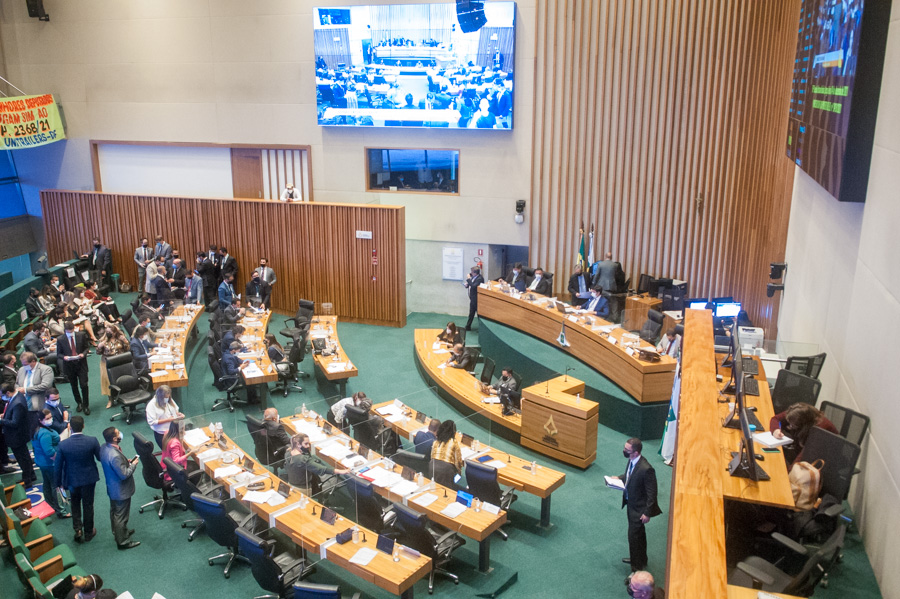
\includegraphics[width=0.5\linewidth]{plenario.jpg}
		\caption{Plenário da Câmara Legislativa do Distrito Federal}
	\end{figure}


\end{frame}
% =========================================================
\section{Experiments conducted} %21
\begin{frame}
	\frametitle{Experiments conducted}
	\framesubtitle{Understanding the experiments}
	
	\begin{block}{The experiments} 
		\scriptsize
		
		\begin{itemize}
			\item In all experiments, a cross-validation with three stratified partitions is performed.
			
			\item The three partitions are randomly divided in a way that it allows training and testing each model for all four metrics, both for training and testing data.
			
			\item In addition to the four metrics, the training and inference times are also measured.
			
			\item For each metric, we get the average of the three validations.  
			
			
		\end{itemize}
	\end{block}

	\begin{exampleblock}{Why? To check for overfitting or underfitting} 
	\begin{itemize}
		\item If there is \textbf{good performance in training but not in testing}, there is overfitting.
		
		\item If there is \textbf{poor performance in both training and testing}, there is underfitting.
	\end{itemize}
	\end{exampleblock}
\end{frame}

% ---------------------------------------------------------------

\begin{frame}  %22
	\frametitle{Experiments conducted}
	\framesubtitle{Embedding - Cross Validation}


	\begin{exampleblock}{Embedding Vectorizer} 
		\begin{itemize}
			\item Logistic Regression excels overall. It may not be the best in everything, but across the set of metrics, it is the best.
		\end{itemize}
	\end{exampleblock}

	
	\begin{table}
		\centering
		\resizebox{1\textwidth}{!}{
			\begin{tabular}{lcccccccccc}
\toprule
& fit\_time & score\_time & test\_f1\_weighted & train\_f1\_weighted & test\_balanced\_accuracy & train\_balanced\_accuracy & test\_precision\_weighted & train\_precision\_weighted & test\_recall\_weighted & train\_recall\_weighted \\ 
\midrule
Model &  &  &  &  &  &  &  &  &  &  \\ 
DummyClassifier & 0.028611 & 0.013967 & 0.025819 & 0.025819 & 0.031250 & 0.031250 & 0.014462 & 0.014462 & 0.120258 & 0.120258 \\ 
KNeighborsClassifier & 0.040055 & 1.049414 & 0.307679 & 0.516615 & 0.179927 & 0.370583 & 0.323286 & 0.547667 & 0.311971 & 0.520135 \\ 
\rowcolor{lightgray} LogisticRegression & 3.597823 & 0.025262 & 0.252122 & 0.282075 & 0.217896 & 0.387424 & 0.356856 & 0.397779 & 0.234561 & 0.270780 \\ 
RandomForestClassifier & 225.171689 & 0.825105 & 0.299710 & \textbf{0.807638} & 0.163765 & \textbf{0.865793} & 0.328777 & \textbf{0.835075} & 0.327624 & 0.801934 \\ 
SVM & 42.684947 & 33.030448 & 0.295933 & 0.346580 & \textbf{0.241816} & 0.495388 & \textbf{0.376351} & 0.435997 & 0.276796 & 0.337201 \\ 
XGBClassifier & 253.781450 & 0.560534 & \textbf{0.325231} & 0.800150 & 0.178569 & 0.726839 & 0.330270 & 0.800984 & \textbf{0.341866} & \textbf{0.802977} \\ 
\bottomrule
\end{tabular}

		}
		\caption{Embedding - Cross Validation}
	\end{table}


\end{frame}
% -----------------------------------------------------------
\begin{frame} 
	\frametitle{Experiments conducted}  %23
	\framesubtitle{TfidfVectorizer - Cross Validation}

	\begin{exampleblock}{Tfidf Vectorizer} 
		\begin{itemize}
			\item Once again, Logistic Regression excels overall.
		\end{itemize}
	\end{exampleblock}

	
	\begin{table}
		\centering
		\resizebox{1\textwidth}{!}{
			\begin{tabular}{lcccccccccc}
\toprule
 & fit\_time & score\_time & test\_f1\_weighted & train\_f1\_weighted & test\_balanced\_accuracy & train\_balanced\_accuracy & test\_precision\_weighted & train\_precision\_weighted & test\_recall\_weighted & train\_recall\_weighted \\
\midrule
Model &  &  &  &  &  &  &  &  &  &  \\
DummyClassifier & 0.005016 & 0.013737 & 0.025819 & 0.025819 & 0.031250 & 0.031250 & 0.014462 & 0.014462 & 0.120258 & 0.120258 \\
KNeighborsClassifier & 0.004096 & 28.906825 & 0.323249 & 0.541327 & 0.181929 & 0.396655 & 0.446675 & 0.629905 & 0.299141 & 0.527901 \\
\rowcolor{lightgray} LogisticRegression & 3.725738 & 0.018837 & 0.467718 & 0.584556 & \textbf{0.377732} & 0.727172 & 0.506144 & 0.629863 & 0.458011 & 0.585697 \\
RandomForestClassifier & 267.923079 & 1.148535 & 0.435199 & \textbf{0.806360} & 0.272152 & \textbf{0.864809} & 0.445313 & \textbf{0.834005} & 0.449355 & \textbf{0.801044} \\
SVM & 44.651407 & 12.235956 & \textbf{0.472803} & 0.676972 & 0.319393 & 0.803307 & \textbf{0.512542} & 0.712173 & 0.456292 & 0.673389 \\
XGBClassifier & 102.740959 & 1.606697 & 0.449333 & 0.766095 & 0.277803 & 0.768935 & 0.449830 & 0.767603 & \textbf{0.458809} & 0.769460 \\
\bottomrule
\end{tabular}

		}
		\caption{TfidfVectorizer - Cross Validation}
	\end{table}


\end{frame}
% -----------------------------------------------------------
\begin{frame}
	\frametitle{Experiments conducted}  %24
	\framesubtitle{TfidfVectorizer and MultiOutputClassifier - Cross Validation}

	\begin{exampleblock}{TfidfVectorizer and MultiOutputClassifier} 
		\begin{itemize}
			\item Once again, Logistic Regression proves to be the top-performing model.
		\end{itemize}
	\end{exampleblock}
	
	\begin{table}
		\centering
		\resizebox{1\textwidth}{!}{
			\begin{tabular}{lrrrrrrrrrr}
\toprule
& fit\_time & score\_time & test\_f1\_w & train\_f1\_w & test\_bal\_a & train\_bal\_a & test\_prc\_w & train\_prc\_w & test\_rec\_w & train\_rec\_w \\ 
 \midrule
Model &  &  &  &  &  &  &  &  &  &  \\
DummyClassifier & 0.004188 & 0.011938 & 0.025819 & 0.025819 & 0.031250 & 0.031250 & 0.014462 & 0.014462 & 0.120258 & 0.120258 \\
KNeighborsClassifier & 0.005413 & 29.213731 & 0.323249 & 0.541327 & 0.181929 & 0.396655 & 0.446675 & 0.629905 & 0.299141 & 0.527901 \\
\rowcolor{lightgray} LogisticRegression & 3.685860 & 0.019390 & 0.467718 & 0.584556 & \textbf{0.377732} & 0.727172 & 0.506144 & 0.629863 & 0.458011 & 0.585697 \\
RandomForestClassifier & 268.849362 & 1.154890 & 0.434992 & \textbf{0.806396} & 0.272071 & \textbf{0.864844} & 0.444953 & \textbf{0.834183} & 0.449048 & \textbf{0.800982} \\
SVM & 44.404848 & 12.142895 & \textbf{0.472803} & 0.676972 & 0.319393 & 0.803307 & \textbf{0.512542} & 0.712173 & 0.456292 & 0.673389 \\
XGBClassifier & 102.840638 & 1.657798 & 0.449333 & 0.766095 & 0.277803 & 0.768935 & 0.449830 & 0.767603 & \textbf{0.458809} & 0.769460 \\
\bottomrule
{} \\
\multicolumn{10}{l}{\textbf{Legends:}}   \\ \midrule
\multicolumn{5}{l}{test\_f1\_w: test\_f1\_weighted} & \multicolumn{5}{l}{train\_f1\_w: train\_f1\_weighted} \\
\multicolumn{5}{l}{test\_bal\_a : test\_balanced\_accuracy } & \multicolumn{5}{l}{train\_bal\_a : train\_balanced\_accuracy } \\
\multicolumn{5}{l}{test\_prc\_w : test\_precision\_weighted } & \multicolumn{5}{l}{train\_prc\_w : train\_precision\_weighted } \\
\multicolumn{5}{l}{test\_rec\_w : test\_recall\_weighted} & \multicolumn{5}{l}{train\_rec\_w : train\_recall\_weighted} \\
\end{tabular}

		}
		\caption{TfidfVectorizer and MultiOutputClassifier - Cross Validation}
	\end{table}

\end{frame}
% =========================================================
\section{Results}  %25
\begin{frame}
	\frametitle{Results}
	\begin{columns}
	
	\begin{column}{0.5\textwidth}

		\begin{block}{Results} 
			\begin{itemize}
				\item Logistic Regression trained with TfidfVectorizer and MultiOutputClassifier had the best results.
			\end{itemize}
		\end{block}
	
 	\end{column}
			
	\begin{column}{0.5\textwidth}
		\begin{table}
		\centering
			\resizebox{0.6\textwidth}{!}{
				\begin{tabular}{|c|c|c|c|c|}
\hline
\textbf{Class} & \textbf{Precision} & \textbf{Recall} & \textbf{F1-Score} & \textbf{Support} \\
\hline
0  & 0.11 & 0.08 & 0.10 & 24 \\
1  & 0.45 & 0.43 & 0.44 & 128 \\
2  & 0.48 & 0.33 & 0.39 & 78 \\
3  & 0.07 & 0.16 & 0.10 & 94 \\
4  & 0.18 & 0.34 & 0.24 & 120 \\
5  & 0.50 & 0.14 & 0.21 & 44 \\
6  & 0.00 & 0.00 & 0.00 & 6 \\
7  & 0.38 & 0.12 & 0.19 & 24 \\
8  & 0.23 & 0.21 & 0.22 & 43 \\
9  & 0.49 & 0.38 & 0.43 & 110 \\
10 & 0.50 & 0.13 & 0.21 & 76 \\
11 & 0.19 & 0.11 & 0.14 & 66 \\
12 & 0.68 & 0.69 & 0.69 & 254 \\
13 & 0.23 & 0.16 & 0.19 & 154 \\
14 & 0.48 & 0.57 & 0.52 & 65 \\
15 & 0.59 & 0.64 & 0.62 & 208 \\
16 & 0.83 & 0.75 & 0.79 & 146 \\
17 & 0.52 & 0.27 & 0.35 & 90 \\
18 & 0.44 & 0.25 & 0.32 & 56 \\
19 & 0.27 & 0.10 & 0.15 & 30 \\
20 & 0.00 & 0.00 & 0.00 & 9 \\
21 & 0.47 & 0.45 & 0.46 & 108 \\
22 & 0.60 & 0.20 & 0.30 & 15 \\
23 & 1.00 & 0.20 & 0.33 & 5 \\
24 & 0.68 & 0.45 & 0.54 & 80 \\
25 & 0.53 & 0.80 & 0.63 & 259 \\
26 & 0.48 & 0.57 & 0.52 & 159 \\
27 & 0.53 & 0.43 & 0.48 & 130 \\
28 & 0.33 & 0.14 & 0.20 & 90 \\
29 & 0.60 & 0.66 & 0.63 & 293 \\
30 & 0.20 & 0.07 & 0.10 & 30 \\
31 & 0.42 & 0.48 & 0.45 & 264 \\
\hline
\multicolumn{4}{|c|}{\textbf{Accuracy}} & 0.47 \\
\hline
\multicolumn{4}{|c|}{\textbf{Macro Avg}} & \\
\hline
 & 0.42 & 0.32 & 0.34 & 3258 \\
\hline
\multicolumn{4}{|c|}{\textbf{Weighted Avg}} & \\
\hline
 & 0.48 & 0.47 & 0.46 & 3258 \\
\hline
\end{tabular}

			}
			\caption{Results}
		\end{table}
	\end{column}

\end{columns}
\end{frame}
% =========================================================
\section{Conclusions}  %26
\begin{frame}
	\frametitle{Conclusions}

	\begin{alertblock}{Accuracy Issues}
	\begin{itemize}
		\item The classifications are not representative of the true distribution;
		\item There are insufficient data to meet the desired objectives;
	\end{itemize}
	\end{alertblock}

	\begin{exampleblock}{As a recommendation model}
		\begin{itemize}
			\item \textbf{Top 3 probabilities:} 0.7027
			\item \textbf{Top 4 probabilities:} 0.7613
			\item \textbf{Top 5 probabilities:} 0.8030
		\end{itemize}
	\end{exampleblock}

\end{frame}
% =========================================================
\section{Future Work}  %27
\begin{frame}
	\frametitle{Future Work}
	\begin{block}{Future Work}
		\begin{itemize}
			\item Integrate a neural network model into the experiments;
			\item Refine class definitions and reclassify the data for improved accuracy;
		\end{itemize}
	\end{block}
\end{frame}
% =========================================================
\section*{Agradecimentos}  %28
\begin{frame}
	\frametitle{Thank You}
    \centering
	\Huge
	
	\fontfamily{cmr}\selectfont	
	\textbf{\textsc{Thank You}}
\end{frame}

















